
\documentclass[letter]{moderncv} % Font sizes: 10, 11, or 12; paper sizes: a4paper, letterpaper, a5paper, legalpaper, executivepaper or landscape; font families: sans or roman
\usepackage[margin=30pt]{geometry}
\moderncvstyle{classic} % CV theme - options include: 'casual' (default), 'classic', 'oldstyle' and 'banking'
\moderncvcolor{blue} % CV color - options include: 'blue' (default), 'orange', 'green', 'red', 'purple', 'grey' and 'black'


%\setlength{\hintscolumnwidth}{3cm} % Uncomment to change the width of the dates column
%\setlength{\makecvtitlenamewidth}{10cm} % For the 'classic' style, uncomment to adjust the width of the space allocated to your name

%----------------------------------------------------------------------------------------
%	NAME AND CONTACT INFORMATION SECTION
%----------------------------------------------------------------------------------------

\firstname{} % Title is Misused here
\familyname{}
\title{\textbf{\textcolor{black}{IEEE CTW 2019 -- Positioning Algorithm Competition}}} %Deutsch
%----------------------------------------------------------------------------------------

\pagestyle{empty}

\begin{document}
\thispagestyle{empty}

\includegraphics[width=1\textwidth]{Comsoc}
\maketitle % Print the CV title
\vspace{-4ex}
\section{Background}
%Due to the huge success of mobile communications in almost all areas of modern life, indoor positioning systems   receive large attention from both industry and academia. 
Indoor positioning  is  a key enabler for a wide range of  applications, including   navigation, smart factories and cities, surveillance, security, IoT, and sensor networks. 
Additionally, indoor positioning  can be leveraged for improved beamforming and  channel estimation in wireless communications. 

%Given the impact of IPS, this CTW competition presents a dataset of channel state information obtained for a massive multiple-input multiple-output (MIMO)-orthogonal frequency division multiplex (OFDM) channel sounder [1], for indoor positioning. 


%\bigskip

%\textcolor{red}{If you are allowed to deviate from the original text, one could do as below:}

%\textcolor{red}{Given the rise of machine learning and the abundant amount of data available by wireless systems, user positioning based on wireless systems is receiving significant attention from academia and industry.  User poisoning systems are a key enabler for many applications and concepts like navigation systems, smart cities, security and surveillance, internet of things, etc. Therefore, this CTW competition presents a dataset of channel state information obtained for a massive multiple-input multiple-output (MIMO) channel sounder for indoor positioning [1], hoping that cultivates further algorithmic innovations in this context.}

\section{The Competition and Evaluation Criteria}

The object of the competition is to design and train an algorithm that can determine the position of a user, based
on estimated channel frequency responses between the user  and  an antenna array. 
Possible solutions may build on classic algorithms (fingerprinting, interpolation) or  machine-learning   approaches. 

~

Channel vectors from  a dataset created with the channel sounder in described [1] will be used.  
The dataset comprises channel responses and associated position ground truth information (see below for more detail), and may be partitioned into training and probe sets as found appropriate for
the algorithm development and training.

~

To compete, teams should download the dataset and develop algorithms. 
In the morning of May 28, 2019, at IEEE CTW, a set of test data comprising only channel responses (but no ground truth) will be distributed. 
During the day, the participating teams should run their algorithms on this test data set, and submit their
estimated position coordinates to  
\texttt{data-competition@inue.uni-stuttgart.de} no later than 20.00 (Iceland local time).
The winners will be determined by the organizers, by evaluating and comparing the root-mean-square position error, averaged over all positions in the test
dataset, of the submitted solutions.


\section{Awards}

A 500\$ prize will be awarded to the winning team.
%Each individual person or team is allowed to submit (up to three) solutions (prediction on the h\_Estimated\_Test.mat) to and present their solution on the CTW as a poster. A prize will be given out for the first three candidates.
%The metric for evalation is $\mathrm{E}(|d-\hat{d}|)$, with $\hat{d}$ being the estimated user position.

\section{About the Dataset}

The dataset was acquired by the massive MIMO channel sounder described in [1].
Specifically, channel responses were measured between a moving transmitter and an 8$\times$2 antenna array. 
As transmitter, an SDR-equipped vacuum-cleaner robot was used, and it drove in a random path on a $\sim 4\times 2$ m table and transmitted uplink OFDM pilots with a bandwidth of 20~MHz and 1024 subcarriers at a carrier frequency of 1.25GHz. 10 \% of the subcarriers were used as guard bands.
\vspace{22ex}

~


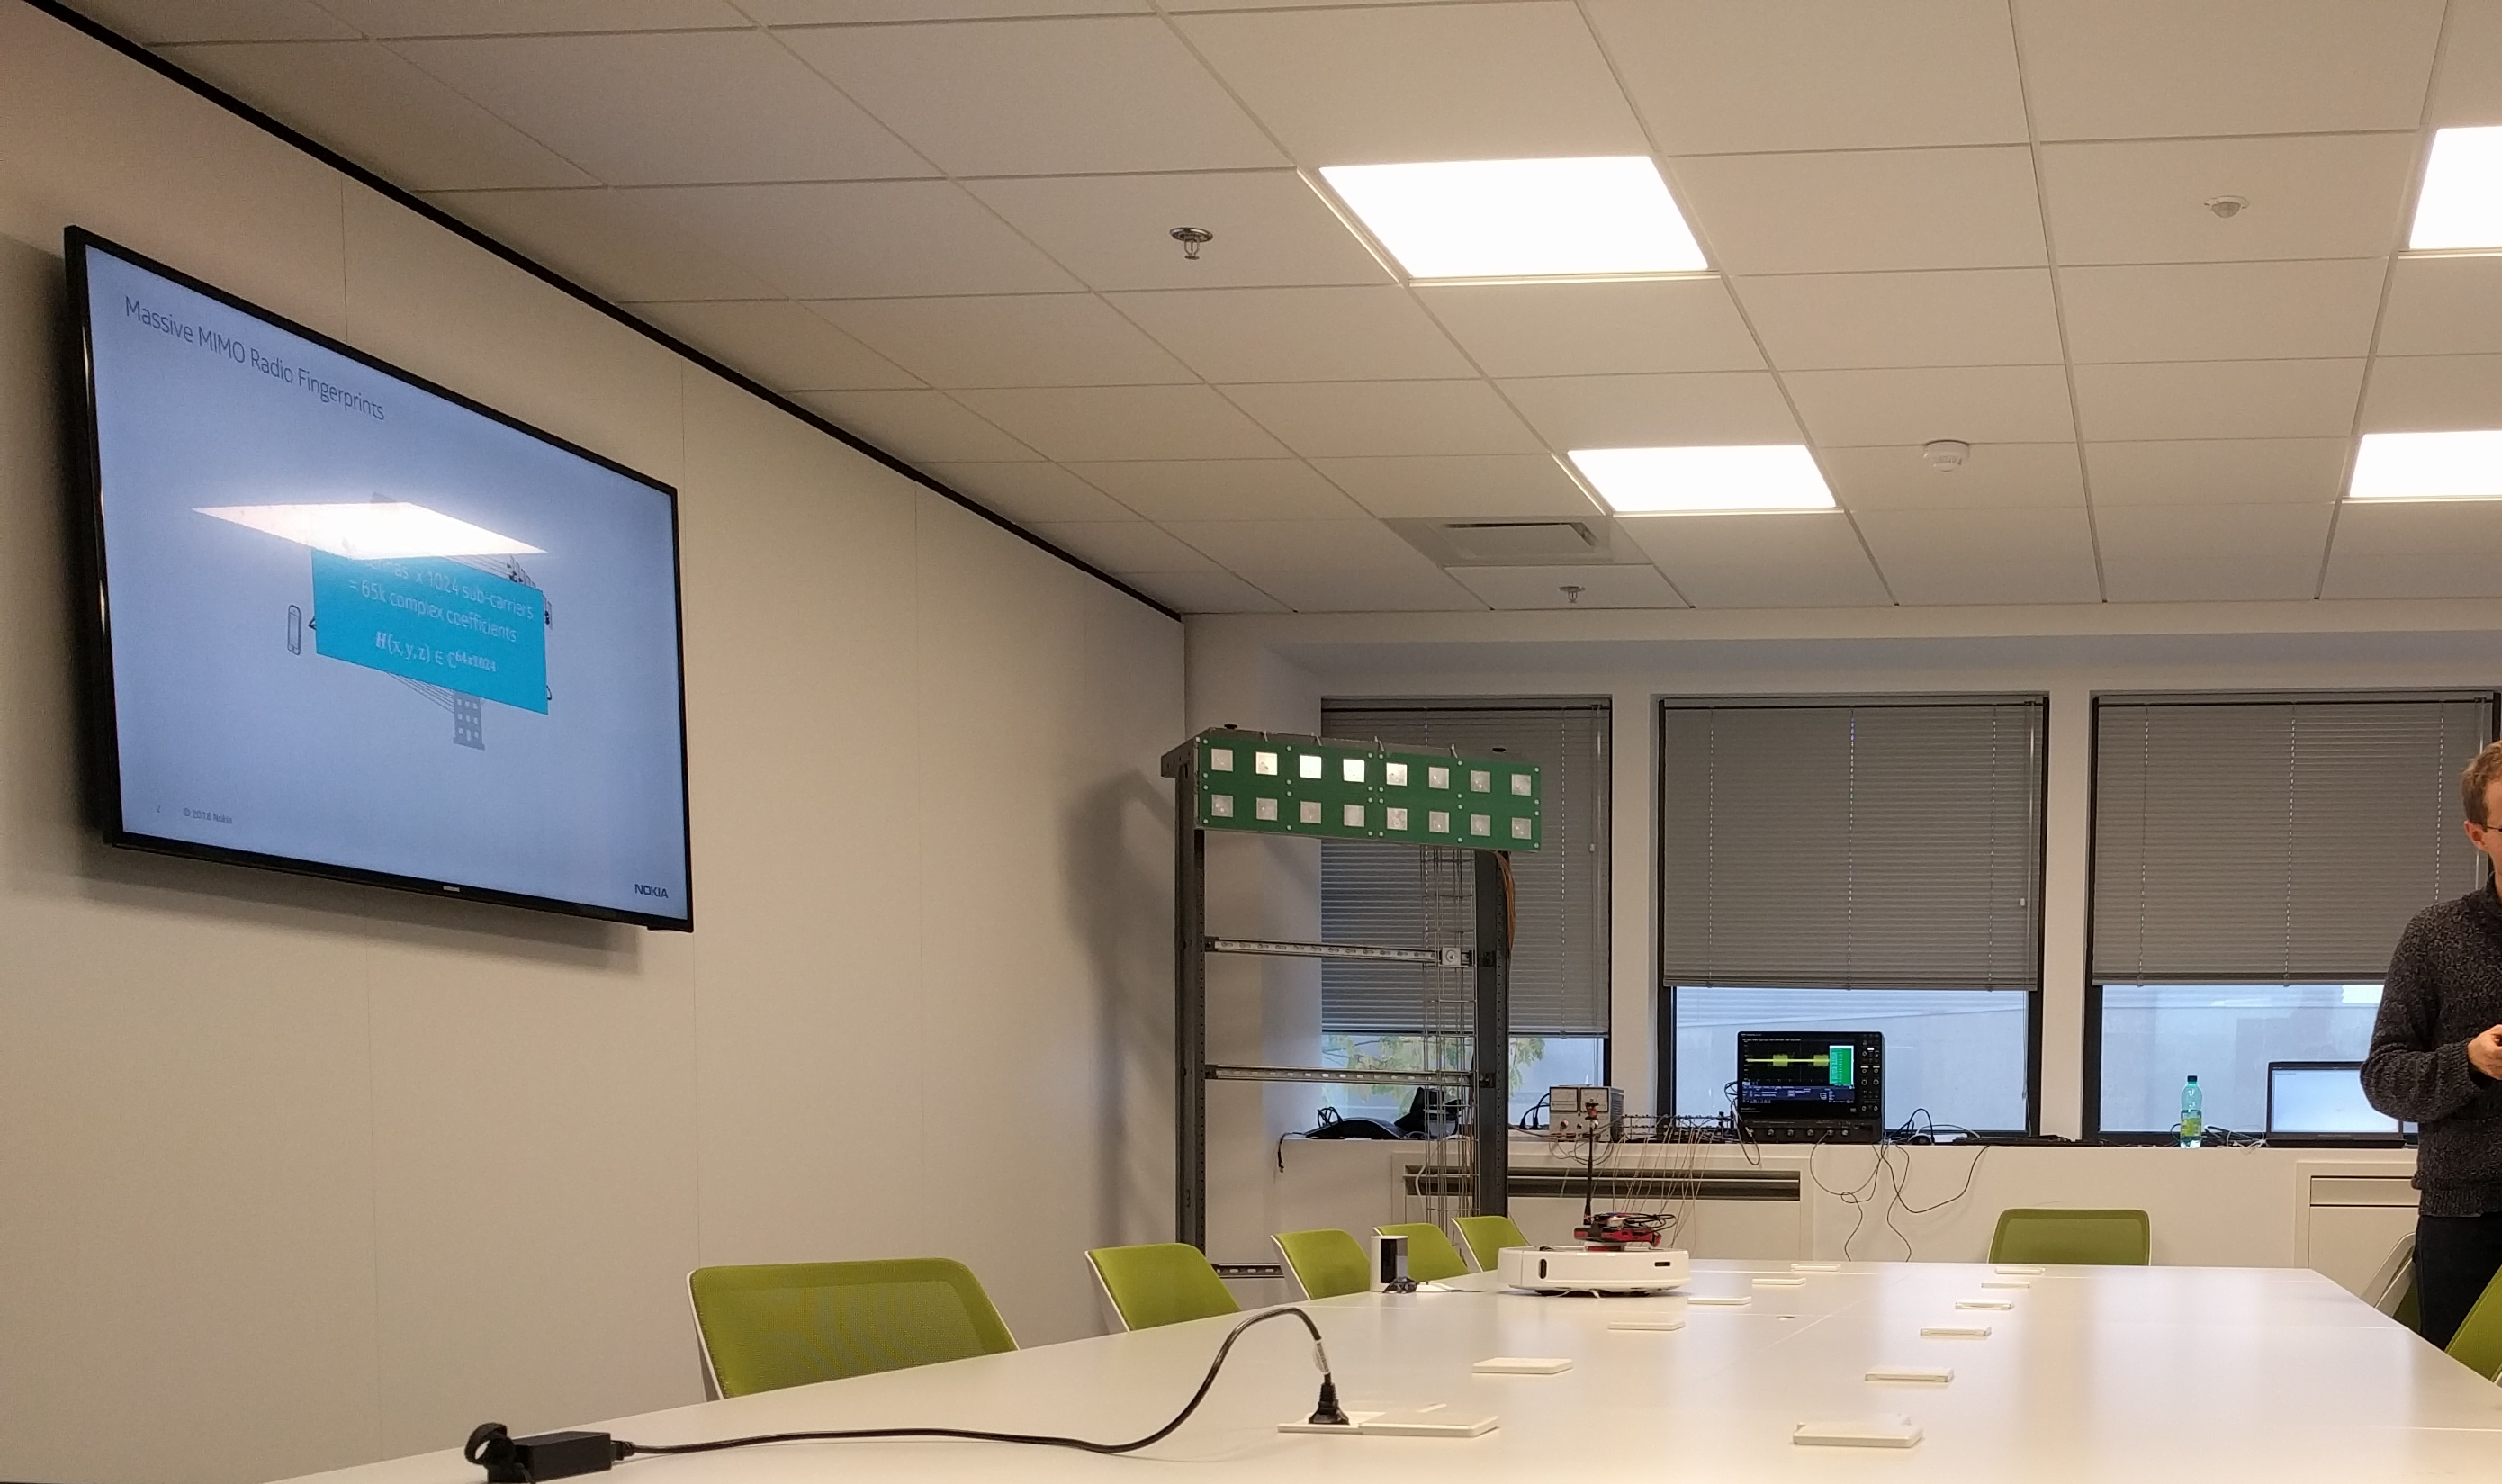
\includegraphics[width=0.5\textwidth]{ParisEnvironment}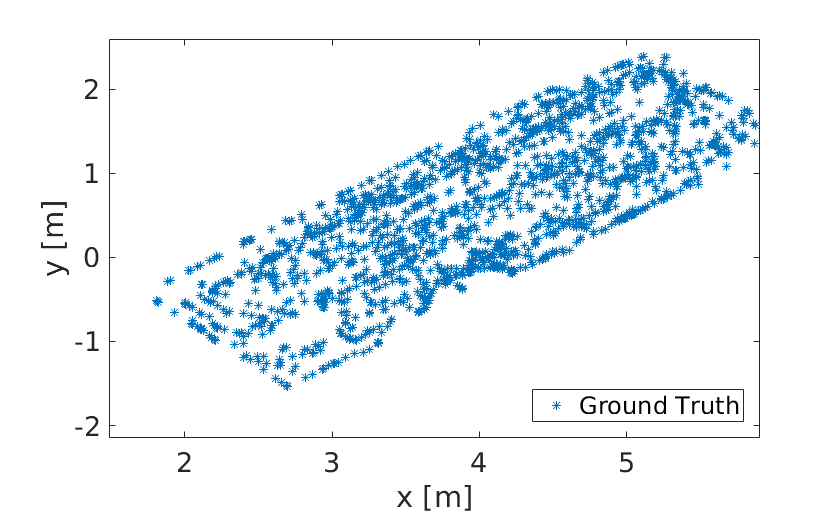
\includegraphics[width=0.5\textwidth]{IndoorDataset}
The left figure shows a picture of the measurement setup. The
right figure shows  an example of  ground truth coordinates, measured by a tachymeter with an accuracy below 1cm.
\vspace{4ex}

 
~

The data are provided in three different formats (.mat, h5, and pickle), and    available via the following links: \newline
  MAT:    \url{https://drive.google.com/open?id=11IGqnn9k8vjkgfMG4G0-AYTgIA5CoDMW} \newline
  HDF;    \url{https://drive.google.com/open?id=11qtImrA8Y12L_2RncRC12GXKo0pdrYhT} \newline
  PICKLE: \url{https://drive.google.com/open?id=1HNXjmyMZe6D828oYuhEQqmW5jwf4wy_I} \newline

~

Each link contains three files:    i) channel responses, ii) ground truth positions, and iii) SNR information.   
The channel variable is called \texttt{h\_Estimated} with the dimension of [Number of measured Points $\times$ Number of antennas (16) $\times$ Number of used subcarriers (924)]. The position is given in the \texttt{r\_Position} variable with dimensions of the number of points  and the coordinates [$x,y,z$] (in this order). The last variable contains the SNR of each antenna at each point resulting in the dimensions 
of [Number of measured Points $\times$ Number of antennas].

~

Further details are available in  the   README file and   Jupyter Notebook provided at the following GitHub page:\newline
\url{https://github.com/MaximilianArnold/CTW2019-PositioningCompetition} \\
This GitHub page also contains an FAQ that will be continuously updated.

 
\pagestyle{empty}


\section{Reference}%
[1] Maximilian Arnold, Jakob Hoydis, and Stephan ten Brink,  ``Novel Massive MIMO Channel Sounding Data applied to Deep Learning-based Indoor Positioning'', submitted to SCC2019, arXiv:1810.04126.

\section{Contact}

\begin{itemize}
\item Questions about the dataset: \\
-- Maximilian Arnold, \texttt{maximilian.arnold@inue.uni-stuttgart.de} \\
-- Prof. Stephan ten Brink, \texttt{tenbrink@inue.uni-stuttgart.de} \\

\item General questions about the CTW competition: \\
-- Prof. Erik G. Larsson, \texttt{erik.g.larsson@liu.se} (2019 IEEE CTW technical co-chair) \\
-- Prof. Urbashi Mitra, \texttt{ubli@usc.edu} (2019 IEEE CTW technical co-chair) 

\end{itemize}

%\vspace{65ex}
\vfill


\includegraphics[width=1\textwidth]{Comsoc}

\end{document}
